\chapter{Stability Conditions}\label{chap:stabilities}
\def\semi{\angle\!}
\newcommand{\thin}{\asymp}
\def\cab{\CC_{[a,b)}}
\def\R{\mathbb{R}}
\def\eps{\varepsilon}
\def\sl{\text{\japanese{切}}}
\todo[inline, caption={}]{
	\begin{itemize}
\item Manca la def di cat artiniana/noetheriana;
\item Manca la definizione di spicing e quella sezione è molto disordinata
	\end{itemize}
}
\section{Introduction}
\epigraph{The cleanest cut is the one you withhold}{???}
The notion of \emph{Bridgeland stability}\footnote{There is an unavoidable clash of notation leading us to refer to stability conditions\index{Stability conditions} with words that allude to a connection between (geometric) stability and the abstract notion of stability for a category. We underline here that nothing, in the following discussion, is written to purport this analogy.} comes from theoretical Physics, and was proposed by T\@. Bridgeland in order to better understand a construction in String Theory, the so\hyp{}called \emph{$\Pi$\hyp{}tability} of \cite{douglas2002dirichlet,douglas2001d}; Bridgeland showed that this notion has a natural interpretation in the language of triangulated categories (the idea of identifying objects of the derived category of sheaves on a space with physical D\hyp{}branes dates back to the work of Moore and Harvey \cite{harvey1998algebras}). 

The main result exposed in \cite{Brid,Bridge2} is that the set of all stability conditions on a given triangulated category $\cate{T}$ can be endowed with a topology, induced by a generalized metric. This allows one to define interesting geometric structures out from a triangulated category.

Up to now, a great effort has been put (sometimes, unfortunately, to no avail), in producing spaces of stability conditions attached to derived categories of certain algebraic varieties, and to study some of their geometric properties; at the moment of writing, a general theory of these spaces is missing\footnote{See \cite{Bridge2}, where the author says:
\begin{quote}
there is some yet\hyp{}to\hyp{}be discovered construction that will allow one to define interesting geometric structures on these spaces. \omissis the agreement between spaces of stability conditions and moduli spaces of conformal field theories is impressive enough to suggest that stability conditions do indeed capture some part
of the mathematics of string theory. My own feeling is that at some point in the near future the notion of a stability condition will be subsumed into some more satisfactory framework.
\end{quote}
The present chapter is a --clumsy or not, the reader will decide-- first step towards this more satisfactory framework.}

The main aim of the present note is to re\hyp{}enact the classical theory of \cite{Brid} in the frame of stable $\infty$\hyp{}categories. In this respect, this is one of the important chapter of the present thesis, as it constitutes one of the main application of the language initiated by the ``Rosetta stone'' theorem \refbf{thm:rosetta}. Nevertheless, we only concentrate on a single piece of the rather vast theory of stability conditions on categories, showing that given two ``close enough'' stability functions $Z$ and $W$ and a slicing $J$ compatible with $Z$ then there exist a slicing compatible with $W$, close enough to $J$. A more detailed  recovering of other major results about the space of stability conditions will be hopefully discussed in a forthcoming article \cite{infty-stab}.

Bridgeland's theory exploits some peculiar\footnote{Peculiar to the standard topological structure of the set of real numbers, but not fully essential: see \cite{GKR} for an enlightening ``formal theory of stability functions'', which has been a constant source of inspiration for the present chapter.} properties of increasing families of $t$\hyp{}structures on a triangulated category $\CC$, indexed by the set of real numbers, \ie monotonic functions $\mathbb R\to \textsc{ts}(\CC)$; we paved the way for this definition in our \achap \refbf{chap:hearts}.

\index{Slicing}These collections are called ($\mathbb R$\hyp{}\emph{slicings} in the stable setting; an extremely remarkable result, hidden in Bridgeland's original formulation and made clear by the torsio\hyp{}entric perspective, is the folloiwng:
\begin{quote}
simple topological properties of $\mathbb R$ (completeness as a metric space, properties of the standard euclidean topology and of the topology of lower convergence generated by the base $\{[a,b)\mid a,b\in\mathbb Q\}$\dots) reflect into categorical properties of slicings 
\end{quote}
A deeper analysis of this phenomenon occupies \S\refbf{slici}.
\begin{notat}\label{assumpts}
We follow a number of blanket assumptions all along the chapter: $\CC$ is, as always, a stable $\infty$\hyp{}category, and $\tee$ is a $t$\hyp{}structure on $\CC$; we often demand that $\CC$ is cocomplete, and $\tee$ is left, right or two\hyp{}sided complete. If $J\colon \mathbb{R}\to \ts(\CC)$ is a slicing, we define $\hrt_t=\CC_{[t,t+1)}$; the collection $\{\hrt_t\}$ is called the \emph{heart} of the slicing. The set of slicings $J\colon \R\to \fs(\CC)$ is denoted $\sl_{\R}(\CC)$\footnote{The Japanese verb {\japanese{切る}} (``kiru'', \emph{to cut}) contains the radical {\japanese{切}}, the same of \emph{katana}.}. The real line has to be thought as a time\hyp{}axis, in such a way that a slicing consists of ``a collection of cuttings at prescribed time''; the value of the slicing $J$ at time $\lambda$, $J(\lambda)  =(\CC_{\ge\lambda}, \CC_{<\lambda})$, will be often called the \emph{slice at time $\lambda$}, or the \emph{$\lambda$\hyp{}slice} of $J$.
\end{notat}
We will make frequent use of the following two definitions of an \emph{artinian} and \emph{noetherian} $\infty$\hyp{}category:
\index{Artinian category}
\begin{definition}\label{artinnoether}%[Artinian\fshyp{}noetherian $\infty$\hyp{}category]
A $\infty$\hyp{}category $\CC$ is called
\begin{itemize}
\item \emph{artinian} if for each object $A\in\CC$ there is no infinite ascending chain of subobjects of $A$;
\item \emph{noetherian} if for each object $A\in\CC$ there is no infinite descending chain of quotients of $A$;
\item \emph{of finite length} (or simply \emph{finite}) when it is artinian and noetherian.
\end{itemize}
\end{definition}
\section{Slicings}\label{slici}
\epigraph{Cutting in time\dots Do yo truly believe that the way of the sword is so trivial?}{Kam\=\i zumi Nobutsuna}
\begin{definition}[Suprema and infima]\label{sup-n-inf}
For any object $A$ of $\CC$ we set
\begin{align*}
\sup(A) &=\inf\{\lambda\in \R: A\in \CC_{<\lambda}\};\\
\inf(A) &=\sup\{\lambda\in \R: A\in \CC_{\geq\lambda}\}
\end{align*}
with the convention $\sup(0)=-\infty$ and $\inf(0) = +\infty$ (if $\CC$ is \emph{left\fshyp{}right complete}, \cite[\abbrv{Def} \textbf{1.2.1.19}]{LurieHA}, these are the only objects such that $\sup(X)$ and $\inf(X)$ is not finite).\index{sup-e-inf@$\sup$ and $\inf$}
\end{definition}
\begin{remark}\label{rem.bounds}
It follows directly from the definition that $A\in \CC_{\geq \mu}$ implies $\inf(A)\geq \mu$ and $A\in \CC_{<\mu}$ implies $\sup(A)\leq \mu$. In particular, if $A\in \cab = \CC_{\ge a}\cap \CC_{<b}$ then $a\leq\inf(A)$ and $\sup(A) < b$.
\end{remark}
\begin{lemma}\label{lemma.maggiore.minore}
If $\inf(A)> \mu$ then $A\in \CC_{\geq \mu}$ and if $\sup(A)<\mu$ then $A\in \CC_{<\mu}$. In particular, it follows that for any $A\neq 0$ one has $\inf(A)\leq \sup(A)$ and $A\in \CC_{[\inf(A),\sup(A))}$.
\end{lemma}
\begin{proof}
If $\inf(A)> \mu$ there exists $\lambda_\mu>\mu$ such that $A\in\CC_{\geq \lambda_\mu}$. Since $\lambda_\mu>\mu$, one immediatley gets $A\in\CC_{\geq \mu}$. The proof for $\sup(A)$ is analogous. It follows from this that $A\in \bigcap_{\mu<\inf(A)}\CC_{\geq \mu}=\CC_{\geq \inf(A)}$ and $A\in \bigcap_{\mu>\sup(A)}\CC_{<\mu}=\CC_{\geq \sup(A)}$. If $A\neq 0$ this gives $\CC_{\geq \inf(A)}\cap \CC_{\geq \sup(A)}\neq \{0\}$ and so $\inf(A)\leq \sup(A)$ and $A\in\CC_{[\inf(A),\sup(A))}$. 
\end{proof}
This proves that the two inequalities $a\le \inf(A)$ and $\sup(A) < b$ form a chain:
\begin{corollary}\label{cor.estimates}
Let $A\in \cab$ be a nonzero object. Then $a\leq \inf(A)\leq \sup(A) < b$.
\end{corollary}
An important result links together the contractibility of mapping spaces $\CC(X,Y)$ and suitable inequalities between infima and suprema of co\fshyp{}domains of these maps.
\begin{lemma}\label{lem.zero.morphism}
If $\inf(X)>\sup(Y)$ then $\CC(X,Y)=\{0\}$.
\end{lemma}
\begin{proof}
Let $t\in \R$ be such that $\sup(Y)<t<\inf(X)$. Then $X\in \CC_{\geq t}$ and $Y\in \CC_{<t}$, by Lemma \refbf{lemma.maggiore.minore}; the object\fshyp{}orthogonality of classes in the slice at time $t$ allows to conclude.
\end{proof}
The situation is depicted as follows: there is a ``natural direction'' in which nonzero morphisms of $(\CC,J)$ go: if $\inf(X)$ is greater than $\sup(Y)$, then $Y$ only receives zero morphisms from $X$.
%\todo[inline]{Va un poo' aggiustato questo disegno}
\begin{center}
\begin{figure}[H]
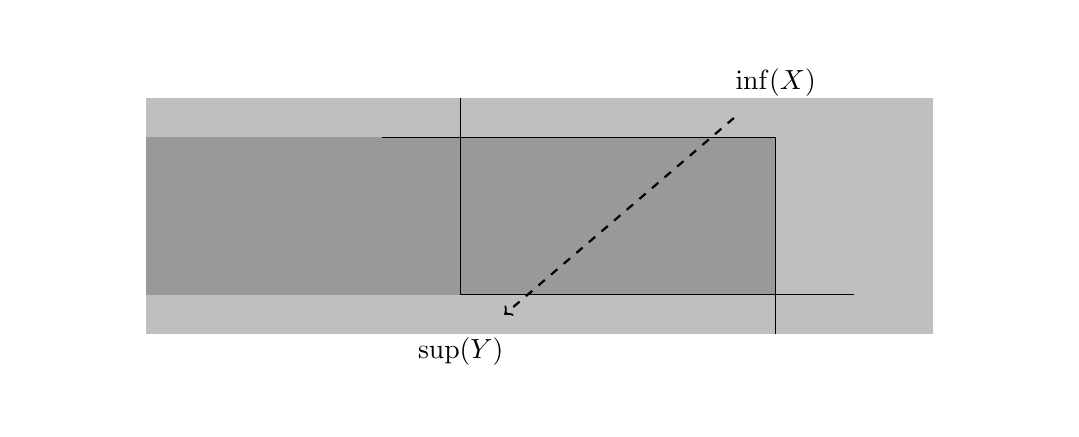
\begin{tikzpicture}
\draw[line width=3cm,lightgray] (-5,0) -- (5,0);
\draw[line width=2cm,gray!80!white] (-5,0) -- (3,0);
\draw[thin] (-2, 1) -- (3,1) -- (3,-1.5);
\draw[thin] (-1, 1.5) -- (-1, -1) -- (4, -1);
\node[circle,above] (sup) at (3,1) {$\inf(X)$};
\node[circle,below] (inf) at (-1, -1) {$\sup(Y)$};
\draw[dashed,thick,->] (sup) -- (inf);
\end{tikzpicture}
% \begin{tikzpicture}
% \draw[thin] (-2, 1) -- (3,1) -- (3,-1);
% \draw[thin] (-1, 1.5) -- (-1, -.5) -- (4, -.5);
% \node[right] at (3,1) {$\inf(X)$};
% \node[left] at (-1, -.5) {$\sup(Y)$};
% \end{tikzpicture}
\caption{Lemma \refbf{lem.zero.morphism}.}
\end{figure}
\end{center}
By opposition, the above Lemma gives the following.
\begin{lemma}\label{lem.opposite}
Let $f\colon X\to Y$ be a nonzero morphism in $\CC$. Then $\inf(X)\leq \sup(Y)$.
\end{lemma}
\begin{remark}
Lemma \refbf{lem.opposite} provides an additional proof of the fact that for a nonzero object $A$ in $\CC$ one has $\inf(A)\leq \sup(A)$. indeed, if $A$ is nonzero, then $\mathrm{id}_A\colon A\to A$ is a nonzero morphism.
\end{remark}
\begin{lemma}\label{lem.exists.morphism}
Let $A$ be an object in $\CC$ and let $\mu<\sup(A)$. Then there exists a nonzero morphism $f\colon A_\mu\to A$ with $\inf(A_\mu)\geq \mu$.  Similarly, if $\mu>\inf(A)$ then there exists a nonzero morphism $f\colon A\to A_\mu$ with $\sup(A_\mu)\leq \mu$.
\end{lemma}
\begin{proof}
Since $\mu<\sup(A)$, we have $\mu\notin\{\lambda\in \R: A\in \CC_{<\lambda}\}$ and so $A\notin \CC_{<\mu} = \CC_{\geq \mu}^\perp$, and so there exists $A_\mu\in \CC_{\geq \mu}$ and a nonzero morphism $F\colon A_\mu\to A$. Since $A\in \CC_{\geq \mu}$, we have $\inf(A)\geq \mu$ by Remark \refbf{rem.bounds}. The proof of the second part of the statement is analogous. 
\end{proof}
\index{Subcategory!thin ---}
\begin{definition}[Thin subcategory]\label{thin.subcat}
The subcategories $\cab$ of a slicing show an extremely peculiar behaviour when $[a,b)$ is a ``sufficiently small'' interval: we call every such $\cab$ a \emph{thin} subcategory, having in mind \cite[\adef \textbf{7.2}]{Brid}; alternatively $[a,b)$\hyp{}endocardium of the slicing $J$(the reason for this quaint choice of notation is explained in \S\refbf{hearts.endocar}).
\end{definition}
\begin{lemma}\label{lem:thin_are_closed}
Let  
 \[
\begin{kD}
\lattice[mesh={4em}{4em}]{
  \obj A; & \obj B; \\
  \obj 0; & \obj C; \\
};
\mor A -> B -> C;
\mor * -> 0 -> *;
\pullout{A}{C};
\end{kD}
 \]
be a fiber sequence in $\CC$ with $A,B$ and $C$ in $\cab$ with $b-a\leq 1$. Then $\sup(A)\leq \sup(B)$ and $\inf(B)\leq \inf(C)$.
\end{lemma}
\begin{proof}
We only prove $\sup(A)\leq \sup(B)$ , the other proof being specular. Assume $\sup(A)>\sup(B)$. Then there exists $\mu$ with $\sup(A)>\mu>\sup(B)$ and so by Lemma \refbf{lem.exists.morphism} there exists a nonzero morphism $f\colon A_\mu\to A$, with $\inf(A_\mu)\geq \mu>\sup(B)$. By Lemma \refbf{lem.zero.morphism}, the composition $A_\mu\xrightarrow{f} A\to B$ is zero, and so (by the universal property of and by the 2-out-of-3 law for the pullback) the morphism $f$ factors through $C[-1]$. Since the composition $f\colon A_\mu\to C[-1]\to A$ is nonzero, so is the morphism $A_\mu\to C[-1]$, and so by Lemma \refbf{lem.opposite} $\sup(B)<\inf(A_\mu)\leq \sup(C[-1])=\sup(C)-1$. This gives $|\sup(B)-\sup(C)|>1$. On the other hand, since $B,C\in \cab$, by Corollary \refbf{cor.estimates}, both $\sup(B)$ and $\sup(C)$ lie in the interval $[a,b]$ and so $|\sup(B)-\sup(C)|\leq |a-b|\leq 1$.
\end{proof}
 \begin{remark}\label{good_inequalities} Lemma \refbf{lem:thin_are_closed} in particular implies that, if $b-a\leq 1$ and 
   \[
\begin{kD}
\lattice[mesh={4em}{4em}]{
  \obj A; & \obj B; \\
  \obj 0; & \obj C; \\
};
\mor A -> B -> C;
\mor * -> 0 -> *;
\pullout{A}{C};
\end{kD}
 \]
is a fiber sequence with vertices in $\mathbf{C}_{[a,b)}$ and with $B\in \mathbf{C}_{[\tilde{a},\tilde{b})}$, for some $a\leq \tilde{a}<\tilde{b}\leq b$, then $A\in \mathbf{C}_{[a,\tilde{b})}$ and $C\in \mathbf{C}_{[\tilde{a},b)}$. 
\end{remark}
We also record a direct proof of this fact, independent from \refbf{lem:thin_are_closed}. Consider the pasting of pullout diagrams
\[
\begin{kD}
\lattice[mesh]{
	& \obj C[-1]; & \obj (01):0;\\
	\obj (Abb):A_{[\tilde{b},b)}; & \obj A; & \obj B; \\
	\obj (02):0; & \obj (Aab):A_{[a,\tilde{b})}; & \obj K;\\
	&\obj 0; & \obj C; \\
};
\mor C[-1] -> 01 -> B -> K -> C;
\mor C[-1] -> A <- Abb -> 02 -> Aab -> 0 -> C;
\mor B <- A -> Aab -> K;
\end{kD}
\]
Since $A_{[\tilde{b},b)}$ is in $\CC_{[\tilde{b},b)}$ and $B\in \CC_{[\tilde{a},\tilde{b})}$, the morphism $A_{[\tilde{b},b)}\to A\to B$ is the zero morphism and so $A_{[\tilde{b},b)}\to A$ factors through $C[-1]$. But $C[-1]\in \CC_{[a-1,b-1)}$ and $b-1\leq a<\tilde{b}$, so that $\CC(A_{[\tilde{b},b)}, C[-1])=0$. 

This implies that $A_{[\tilde{b},b)}\to A$ is the zero morphism, and so $A_{[\tilde{b},b)}=0$ and $A=A_{[a,\tilde{b})}$. The proof for $C$ is specular.
\begin{proposition}
If $X\in \CC_{[0,1)}\setminus \CC_{\{0\}}$, then there is a nonzero morphism $Y_\eps\to X$ for some $\eps > 0$ and $\bar Y\in \CC_{[\eps,1)}$.
\end{proposition}
\begin{proof}
It is immediate to notice that if $X\in \CC_{[0,1)} \setminus \CC_{0}$, then there exists an $\eps > 0$ such that $X\notin \CC_{[0,\eps)}$, so $X\notin \CC_{[\eps ,+\infty)}^\perp = \CC_{<\eps}$, hence it receives a nonzero morphism $Y_\eps\to X$ from an object $Y_\eps\in \CC_{[\eps,+\infty)}$; now $\fF_1$\hyp{}factor this morphism: 
\[
Y_\eps\xto{e_1}\bar{Y}\xto{m_1} X; 
\]
the object $\bar{Y}$ now lies in $ \CC_{[\eps,1)}$.
\end{proof}
\subsection{A topology on slicings}
\index{Slicing!topology on ---}
In \cite{Brid} the author defines a generalized metric (and hence a topology) on the set $\text{Stab}(\D)$ of stability conditions on the triangulated category $\D$; now, we show that this definition corresponds, in the torsio\hyp{}centric approach, to a generalized metric (and hence a topology) on the set of slicings.
\subsubsection{A metric on $\sl_\mathbb{R}(\CC)$}
\begin{definition}\label{this.is.the.metric}
\index{Slicing!metric on ---}
Let $I$ and $J$ two slicings on $\CC$ and denote by $(\CC_{<t}^I,\CC_{\geq t}^I)$ and $(\CC_{<t}^J,\CC_{\geq t}^J)$ the corresponding families of $t$\hyp{}structures. We set
\[
d(I,J)=\inf\{\eps >0 \mid \CC_{<t}^I\subseteq \CC_{<t+\eps}^J \text{ and } \CC_{\geq t}^I\subseteq \CC_{\geq t-\eps}^J \text{ for any } t\in \R\}.
\]
This defines a function
\[
d\colon \sl_{\R}(\CC) \times \sl_{\R}(\CC) \to [0,+\infty]
\]
\end{definition}
\begin{remark}\label{rem.reformulation}
One can equivalently define $d$ as 
\[
d(I,J)=\inf\{\eps >0 \mid \CC_{\geq t}^J\subseteq \CC_{\geq t-\eps}^I \text{ and } \CC_{\geq t}^I\subseteq \CC_{\geq t-\eps}^J \text{ for any } t\in \R\}.
\]
Namely, the condition $\CC_{<t}^I\subseteq \CC_{<t+\eps}^J$ is equivalent to $\CC_{\geq t}^{I,\perp}\subseteq \CC_{\geq t+\eps}^{J,\perp}$ and so to $\CC_{\geq t+\eps}^{J}\subseteq 
\CC_{\geq t}^{I}$. Since this has to hold for every $t$, this is equivalent to $\CC_{\geq t}^{J}\subseteq 
\CC_{\geq t-\eps}^{I}$. 
\end{remark}
We split the proof that the function $d$ is a metric on $\sl_\mathbb{R}(\CC)$ in lemma \refbf{lem.symmetry}, \refbf{lem.zero.distance}, \refbf{lem.triangle.ineq} below.
\begin{lemma}\label{lem.symmetry}
The function $d$ is symmetric.
\end{lemma}
\begin{proof}
Manifest from the expression for $d$ given in Remark \refbf{rem.reformulation}.
\end{proof}
\begin{lemma}\label{lem.finite.distance}
If $d(I,J)$ is finite, then $\CC_{\geq t}^{I}\subseteq \CC_{\geq t-d(I,J)}^{J}$ and $\CC_{\geq t}^{J}\subseteq \CC_{\geq t-d(I,J)}^{I}$, for any $t\in \R$.
\end{lemma}
\begin{proof}
Let $t_0\in \R$. By definition of $d$ and by Remark \refbf{rem.reformulation}, for any $\eps>0$ there exists $\delta$ with $d(I,J)\leq \delta<d(I,J)+\eps$ such that $\CC_{\geq t}^J\subseteq \CC_{\geq t-\delta}^I$ and $\CC_{\geq t}^I\subseteq \CC_{\geq t-\delta}^J$ for any $t\in \R$. In particular this implies $\CC_{\geq t_0}^J\subseteq \CC_{\geq t_0-d(I,J)-\eps}^I$ and $\CC_{\geq t_0}^I\subseteq  \CC_{\geq t_0-d(I,J)-\eps}^J$. Since this holds for any $\eps>0$, we get $\CC_{\geq t_0}^J\subseteq \CC_{\geq t_0-d(I,J)}^I$ and $\CC_{\geq t_0}^I\subseteq  \CC_{\geq t_0-d(I,J)}^J$. Since $t_0$ was arbitrary, this concludes the proof.
\end{proof}
\begin{lemma}\label{lem.zero.distance}
One has $d(I,J)=0$ if and only if $I=J$.
\end{lemma}
\begin{proof}
Clearly, if $I=J$ then $d(I,J)=0$. Conversely, assume $d(I,J)=0$. Then, by Lemma \refbf{lem.finite.distance}, we get $\CC_{\geq t}^J\subseteq \CC_{\geq t}^I$ and $\CC_{\geq t}^I\subseteq  \CC_{\geq t}^J$, i.e., $\CC_{\geq t}^I=\CC_{\geq t}^J$, for any $t\in\R$.
\end{proof}
\begin{lemma}\label{lem.triangle.ineq}
The function $d$ satisfies the triangular inequality, i.e., for any three slicings $I,J,K$ one has
\[
d(I,K)\leq d(I,J)+d(J,K)
\]
\end{lemma}
\begin{proof}
If either $d(I,J)$ or $d(J,K)$ are infinite then there is nothing to prove. Assume then that both $d(I,J)$ and $d(J,K)$ are finite. By Lemma  \refbf{lem.finite.distance}, for any $t\in \R$ we have $\CC_{\geq t}^{I}\subseteq 
\CC_{\geq t-d(I,J)}^{J}\subseteq \CC_{\geq t-d(I,J)-d(J,K)}^{K}$ and $\CC_{\geq t}^{K}\subseteq \CC_{\geq t-d(J,K)}^{J}\subseteq \CC_{\geq t-d(J,K)-d(I,J)}^{I}$.
\end{proof}
%\subsection{A topology on $\sl_\mathbb{R}(\CC)$}
We now define\fare
\begin{definition}\label{this.basis}
Let $\eps > 0$ a real number and $J\colon \R\to \fs(\CC)$ be a slicing; we define
\[
U_\eps(J) = \big\{ \tilde{J}\colon \R\to \fs(\CC)\mid \exists \delta : (\forall t\in\R)\;\EE_{t+\eps} \subseteq \tilde{\EE}_{t+\delta} \subseteq \tilde{\EE}_{t-\delta} \subseteq \EE_{t-\eps} \big\}
\]
where $\EE_\lambda$ is the left class of $J(\lambda)$, and similarly $\tilde{\EE}_\lambda$ is the left class of $\tilde{J}(\lambda)$ for each $\lambda\in\mathbb R$.
\end{definition}
\begin{proposition}\label{is.a.basis}
The set $\mathcal{U}= \{U_\eps(J)\mid \eps > 0, \; J\in \sl_{\R}(\CC)\}$ forms a basis for a topology $\tau_{\mathcal U}$ on $\sl_{\R}(\CC)$.
\end{proposition}
\begin{proof}
As always, we have to prove that 
\begin{enumerate}
\item The family $\mathcal{U}$ forms a covering of $\sl_{\R}(\CC)$;
\item every nonempty intersection $U_\alpha(J_1)\cap U_\beta(J_2)$ containing $I$ contains also a basis element containing $I$.
\end{enumerate}
The first point is obvious, as every $J\in \sl_{\R}(\CC)$ lies in $U_\eps(J)$ for $\eps > 0$.

Now, if $J\in U_\alpha(J_1)\cap U_\beta(J_2)$ for $J_1,J_2\in\sl_{\R}(\CC)$ and $\alpha,\beta > 0$, then we have inequalities
\begin{gather*}
\EE^1_{t-\alpha} \supseteq \EE_{t-\delta_1} \supseteq \EE_{t+\delta_1} \supseteq \EE^1_{t+\alpha}\\
\EE^2_{t-\beta} \supseteq \EE_{t-\delta_2} \supseteq \EE_{t+\delta_2} \supseteq \EE^2_{t+\beta}
\end{gather*}
for suitable $\delta_1,\delta_2 > 0$; it is enough to choose $\gamma > 0$ such that the inequalities
\[
\EE_{t+\delta_1} \subseteq \EE_{t+\gamma} \subseteq \EE_{t-\delta_1} \quad\text{and}\quad 
\EE_{t+\delta_2} \subseteq \EE_{t+\gamma} \subseteq \EE_{t-\delta_2}
\]
both hold: once this choice has been made, every other $\tilde{J} \in U_\gamma(J)$ satisfies $\EE_{t+\gamma}\subseteq \tilde{\EE}_{t+\delta} \subseteq \tilde{\EE}_{t-\delta} \subseteq \EE_{t-\gamma}$ and hence belongs to $U_\alpha(J_1)\cap U_\beta(J_2)$. Any $\gamma < \min\{\delta_1,\delta_2\}$ does the job.
\end{proof}
\begin{proposition}
The topology $\tau_{\mathcal U}$ on $\sl_{\R}(\CC)$ is induced by the metric of Definition \refbf{this.is.the.metric}.
\end{proposition}
\begin{proof}
\todo[inline]{Every basis element is union of balls, every ball is union of open elements.}
\end{proof}
% Un remark dislocato: vorrei prendere non un $\delta$ a caso, ma l'inf di tali $\delta$; ciò crea problemi quando tale inf è zero, però per il momento non pensiamoci.

% Se non altro perché, se tale inf $\delta_0$ è $<\eps$, il remark \refbf{lem.finite.distance} assicura che ogni $I\in U_\eps(J)$ sta anche in $B_d(J, \eps[$.
\begin{proposition}
Let $J\in \sl_{\R}(\CC)$ be a slicing on an \emph{artinian} (see \adef \refbf{artinnoether}) stable $\infty$\hyp{}category, and let $0\le b-a < 1$ be real numbers; then $\bigcap_{\eps > 0} \CC_{[a-\eps,b)} = \cab$.
\end{proposition}
\begin{proof}
It is enough to prove the result when $a=b$, and the only non\hyp{}obvious inclusion is $\bigcap_{\eps > 0} \CC_{[a-\eps,a)} \subseteq (0)$. To prove it, we appeal \abbrv{Prop} \refbf{artinian_implies_internal}: let $X\in \bigcap_{\eps > 0} \CC_{[a-\eps,a)}$; then $X$ belongs \emph{a fortiori} to $\CC_{[a-1,a)}$, and by \abbrv{Prop} \refbf{artinian_implies_internal} there is $z < a$ such that $X\in \CC_{[a-1,z)}$.

Now, choose $\eps_0$ such that $a - \eps_0 > z$ (like for example $\eps_0 = \frac{a-z}{3}$); then $X\in \CC_{[a-\eps_0,a)}\cap \CC_{[a-1,z)} = (0)$.

A similar argument, slightly adapted in an obvious way, gives the result when $0 < b-a < 1$.
\end{proof}
\subsection{Finiteness conditions for slicings}
In the special case where a $t$\hyp{}structure on $\CC$ is ``finite'' in a particular sense, we can perform several other constructions on a slicing $J$: \dots

\index{Spicing}
Spicings form a sub\hyp{}poset of $\sl_\mathbb{R}(\CC)$ denoted $\sl_\mathbb{R}^\textsf{s}(\CC)$.
\begin{definition}[Spicing]\label{spicing}
A \emph{spicing} (also called ``Bridgeland slicing'') is a slicing such that\dots
\end{definition}
\begin{proposition}\label{isaspice}
Let $\R \to \fs(\CC)$ be a spicing, and $t\in \R$ a fixed real number; let
\[\label{eqn:isaspice}
\CC_{>t} \defequal \bigcup_{\eps > 0} \CC_{\ge t+\eps} \quad\text{and}\quad \CC_{\le t} \defequal \bigcap_{\eps >0} \CC_{< t+\eps}.
\]
Then $(\CC_{>t}, \CC_{\le t})$ is a spicing on $\CC$, called the \emph{closure} of $J$ and denoted $\overline J$.
\end{proposition}
\begin{proof}
We have to prove that the pair $(\CC_{>t}, \CC_{\le t})$ forms a $t$\hyp{}structure on $\CC$. Orthogonality is immediate. The presence of a fiber sequence %$X_{>t}\to X\to X_{\le t}$, 
\[
\begin{kD}
\lattice[mesh]{
	\obj (Xge):X_{>t}; & \obj X; \\
	\obj 0; & \obj (Xle):X_{\le t}; \\
};
\mor Xge -> X -> Xle <- 0 <- Xge;
\pullout{Xge}{Xle};
\end{kD}
\]
functorial in the object $X\in \CC$, and such that $X_{>t}\in\CC_{>t}$, $X_{\le t}\in\CC_{\le t}$ can be proved exploiting the completeness exhaustiveness of the slicing: without loss of generality we can construct the fiber sequence $X_{>0}\to X\to X_{\le 0}$ only; it is rather evident how the particular argument adapts to the general case. 

Let $s\in ]0,\eps [$ be a real number, for $0< \eps  \ll 1$ and notice that the arrows $\var{X_{\ge s}}{X}$ and $\var{X}{X_{<s}}$ form diagrams from $\R$ respectively to $\CC/X$ and $X/\CC$.

Thanks to this, we can define 
\[
X_{> 0} \defequal \varprojlim_{s\in ]0,\eps [} \var{X_{\ge s}}{X}\quad\text{and}\quad X_{\le 0} \defequal \varinjlim_{s\in ]0,\eps [} \var{X_{\ge s}}{X}
\]
Universal properties of limits and colimits give a sequence of arrows
\[ X_{>0}\to X\to X_{\le 0}\]
which is a fiber sequence (since\dots) and such that the objects lie in the classes (since \dots). 
\end{proof}
\index{Spicing!closure of ---}
\begin{remark}
The reason to define $\overline{J}$ the ``closure'' of the spicing $J$ is that it behaves like a closure operator $\overline{(-)}\colon \sl_\mathbb{R}^\textsf{s}(\CC) \to \sl_\mathbb{R}^\textsf{s}(\CC)$, namely that for each spicing $J$ one has
\begin{itemize}
\item $\overline{J}\subseteq J$;
\item $\overline{\overline{J}} = \overline{J}$.
\end{itemize}
\end{remark}
See \cite{bondal2013operations} for more information and to uniformize notation. The problem of existence of transfinite intersections is not trivial in view of the notrivial condition for intersecability given there.
\begin{proof}
The first condition is obvious in view of the partial ordering on $\ts(\CC)$: since $\CC_{\ge t+\eps}\subset \CC_{\ge t}$ for each $\eps > 0$, one has $\CC_{>t}\subseteq \CC_{\ge t}$, and passing to the orthogonal $\CC_{\le t}\supseteq \CC_{<t}$; this means that $J\subseteq \overline J$ n the obvious sense.

The second condition amounts to
\[
\bigcup_{\mu > 0}\bigcup_{\eps > 0} \CC_{\ge t+\eps+\mu} = 
\bigcup_{\eps > 0}\CC_{\ge t+\eps};\qquad
\bigcup_{\mu > 0}\bigcup_{\eps > 0} \CC_{< t+\eps+\mu} = 
\bigcup_{\eps > 0}\CC_{ < t+\eps}
\]
which is an obvious set\hyp{}theoretical shenanigan.
\end{proof}
\begin{definition}
A slicing $J\colon \R\to \fs(\CC)$ is said to be \emph{exhaustive} (or $\CC$ is called $J$-\emph{exhaustive}) if the following equality holds:
\[
\bigcup_{t<0}\bigcap_{\eps > 0} \CC_{< t+\eps} = \bigcup_{t<0} \CC_{\le t} = \CC_{<0}.
\]
\end{definition}
A naughty conjecture (probably false): $J$ is a spicing on $\CC$ iff $\CC$ is $J$-exhaustive.

\section{Stability conditions}
\epigraph{MANCA!}{}

% \begin{notat}
% For $A\subseteq \R$, let $K_A\subseteq \mathbb{C}$ denote the cone
% \[
% K_A=\{z\in\mathbb{C}\,|\, z=\rho e^{\pi i \theta} \text{ with } \rho\in \R_{\geq 0} \text{ and } \theta\in A\}.
% \]
% \end{notat}
\index{Stability conditions}
 \begin{definition}\label{la_zeta}
 Let $\CC$ be a stable $\infty$\hyp{}category. A \emph{stability condition} on $\CC$ is a pair $\sigma=(Z,J)$, where:
 \begin{enumerate}[label=\textsc{sc}\oldstylenums{\arabic*})]
 \item $J\colon \R\to \mathrm{ts}(\CC)$ is a \emph{slicing} on $\CC$;
 \item $Z\colon \CC\to \mathbb{C}$ is a functor\footnote{The set $\mathbb{C}$ is seen as the small groupoid having the set $\mathbb{C}$ as set of objects and exactly one arrow between any two objects; because of this, $Z$ is determined by a function $\CC_0\to \mathbb{C}$.}  which factors through the Grothendieck group of $\CC$, i.e., for every fiber sequence 
\[
\begin{kD}
\lattice[mesh={4em}{4em}]{
  \obj A; & \obj B; \\
  \obj 0; & \obj C; \\
};
\mor A -> B -> C;
\mor * -> 0 -> *;
\pullout{A}{C};
\end{kD}
 \]
in $\CC$, one has $Z(A)-Z(B)+Z(C)=0$ (this property is called \emph{additivity} for $Z$);
\item $Z$ is \emph{compatible with the slicing}, \ie for any $a<b$ in $\R$ one has $Z(\cab)\subseteq K_{[a,b)}$. 
\item $Z$ is \emph{nondegenerate on the hearts}, \ie for any $t\in \R$ one has $Z(X)\neq 0$ for any nonzero object of $\hrt_t$.
 \end{enumerate}
\index{Stability function|see Stability conditions}
The functor $Z$ is often regarded as a mere function, and called a \emph{stability function} on $\CC$.
 \end{definition}
 It follows immediately from \textsc{sc}\oldstylenums{2} and \textsc{sc}\oldstylenums{3} that
 \begin{remark}
 The complex number $Z(A)$ only depends on the equivalence class of $A$. Moreover, $Z(A[\pm 1])=-Z(A)$, so that $Z(A[2])=Z(A)$ for any object $A$ in $\CC$.
 \end{remark}
 \begin{remark}
 If one denotes by $\CC_a$ the full subcategory of $\CC$ given by 
 \[
 \CC_a=\bigcap_{\eps>0}\CC_{[a,a+\eps)},
 \]
 then $Z(\CC_a)\subseteq K_{\{a\}}$, \ie $Z(X) = \rho(X) e^{i\pi a}$.
 \end{remark}

\begin{lemma}
Assume $\sigma= (Z,J)$ and $\tau = (Z,I)$ are stability conditions
on $\CC$ with the same central charge $Z$, and with $d(I,J) < 1$. Then $\sigma=\tau$.
\end{lemma}
\begin{proof}
Assume $\sigma\neq \tau$, i.e., that $I\neq J$. Then there exists $t\in\R$ such that $\CC_{\geq t}^I\neq \CC_{\geq t}^J$. Without loss of generality we may assume $\CC_{\geq t}^I\nsubseteq \CC_{\geq t}^J$. On the other hand, by Lemma \refbf{lem.finite.distance}, we have $\CC_{\geq t}^I\subseteq \CC_{\geq t-d(I,J)}^J$ {\it(to be continued\dots)}
\end{proof}

\section{Hearts and endocardia}\label{hearts.endocar}
\epigraph{MANCA!}{}

\index{ab-endocardium@$[a,b)$\hyp{}endocardium}
Slightly adapting the proof of \athm \refbf{heart.is.abelian} it is possible to show that each category $\hrt_\lambda = \CC_{[\lambda,\lambda+1)}$ is abelian; this subcategory is the $\lambda$\emph{\hyp{}heart}, \ie the heart of the slice at time $\lambda$.

We now want to extend the validity of this result to thin (\adef \refbf{thin.subcat}) subcategories $\cab$, by showing (in \abbrv{Thm} \refbf{thm:endocardia_are_ab} below) that all these $\cab$ are abelian $\infty$\hyp{}categories in the sense of \adef \refbf{df:abelinfty}.
\begin{theorem}[Abelianity of endocardia]\label{thm:endocardia_are_ab}
% In every $[a,b)$\hyp{}endocardium each morphism $f\colon X\to Y$ in $\cab$ factors in an essentially unique way as a composition $X\to Z\to Y$, where $Z$ is at the same time a ``subobject'' of $Y$ and a ``quotient'' of $X$.
Every $[a,b)$\hyp{}endocardium is an abelian $\infty$\hyp{}category; it is, in particular, a category with kernel and cokernel functors, respectively $\ker_{[a,b)}$ and $\coker_{[a,b)}$, and this kernels and cokernels fit into pullback and pushout diagrams
\[
\begin{kD}
\lattice[mesh]{
  \obj (S_aF):\ker_{[a,b)}; & \obj X; & \obj (X'):X; & \obj (0'):0; \\
  \obj 0;    & \obj Y; & \obj (Y'):Y; & \obj (R_bC):\coker_{[a,b)}; \\
};
\mor S_aF -> X f:-> Y;
\mor * -> 0 -> *;
\mor X' -> 0' -> R_bC; 
\mor[swap] * f:-> Y' -> *;
\pullback{S_aF}{Y};
\pushout{X'}{R_bC};
\end{kD}
\]
for each $f\colon X\to Y$. There is, moreover, a canonical isomorphism 
\[
\begin{kD}
\lattice[mesh={0em}{12em}]{
\obj (coim):{\coker_{[a,b)}\var{\ker_{[a,b)}(f)}{X}}; & \obj (im):{\ker_{[a,b)}\var{Y}{\coker_{[a,b)}(f)}}; \\
};
\mor coim \simeq:-> im;
\end{kD}
\]
whose domain and codomain are called the \emph{coimage} and \emph{image} of $f$ respectively.
\end{theorem}
\begin{proof}
We re\hyp{}draw the diagram constructed in \refbf{heart.is.abelian}, and reproduce the argument therein: refer to (\refbf{the.diag.of.hearts}) below, 
% \[
% \begin{kD}
% \lattice[mesh={4em}{20mm}]{
%   \obj (ker):\ker_{[a,b)}(f); & \obj F; & \obj X; & \obj (0'):0;\\
%   \obj (0''):0; & \obj (a):\#; & \obj (b):Z; & \obj (c):\#; & \obj (0'''):0;\\  
%   & \obj (0''''):0; & \obj Y; & \obj C; & \obj (coker):\coker_{[a,b)}(f); \\
% };
% \mor ker -> F -> X -> 0' -> c -> C -> coker;
% \mor ker -> 0'' -> a -> b -> c -> 0''' -> coker -> *;
% \mor F -> a -> 0'''' -> Y -> C;
% \mor X -> b -> Y;
% \end{kD}
% \]
where $f\colon X\to Z\to Y$, $F = \fib(f), C = \cofib(f)$ are the fiber and cofiber of $f$, and we refer to $\ker_{[a,b)}(f) = S_a F$ and $\coker_{[a,b)}(f) = R_bC$ as the objects emerging from the ternary factorizations
\[
\xymatrix@R=0mm{
  0 \ar[r] & S_b F\ar[r]  & S_a F\ar[r]  & F \\
  C \ar[r] & R_b C\ar[r]  & R_a C\ar[r]  & 0
}
\]
obtained from the normal torsion theories $\fF_a \preceq \fF_b$. Now, notice that by definition $\ker_{[a,b)}(f) \in \EE_a$ and $\coker_{[a,b)}(f)\in\MM_b$, hence the two objects belong to the $[a,b)$\hyp{}endocardium if and only if $\ker_{[a,b)}(f) \in \MM_b$ and $\coker_{[a,b)}(f)\in\EE_a$. But this easily follows from the fact that $X,Y\in\cab = \EE_a \cap \MM_b$ and from the closure properties of each $\EE_\lambda, \MM_\lambda$: we are in the following situation,% if we write the aove diagram mentioning the class where each arrow belongs, we obtain
\[\label{the.diag.of.hearts}
{\footnotesize \begin{kD}
\lattice[mesh={4em}{22mm}]{
   \obj (ker):\ker_{[a,b)}(f); & \obj F; & \obj X; & \obj (0'):0;\\
   \obj (0''):0; & \obj (a):R_bC[-1]; & \obj (b):Z; & \obj (c):S_aF[1]; & \obj (0'''):0;\\  
  & \obj (0''''):0; & \obj Y; & \obj C; & \obj (coker):\coker_{[a,b)}(f);\\
};
\mor ker m_a:-> F (z0):m_b:-> X {e_a m_b}:-> 0' e_a[1]:-> c m_b:-> C swap:{e_a[1]}:-> coker;
\mor ker swap:e_a:-> 0'' {m_b[-1]}:-> a (z1):m_b:-> b e_a:-> c e_a[1]:-> 0''' m_b:-> coker;
\mor[swap] F e_a:-> a m_b[-1]:-> 0'''' {e_a m_b}:-> Y e_a:-> C;
\mor[swap] X e_a:-> b m_b:-> Y;
\mor[crossing over, gray,near end] X f:r> Y;
\obj at=($(z0)!.5!(z1)$):\boxed{\zeta};
\end{kD}}
\]
and hence, by the closure properties of $\MM_b$ and $\EE_a$, we conclude.
\end{proof}
To conclude the proof we must show that $\ker_{[a,b)}(f)$ and $\coker_{[a,b)}(f)$ indeed have the desired universal properties of kernel and cokernel, namely that in each endocardium the diagrams
\[
\begin{kD}
\lattice[mesh={4em}{7em}]{
  \obj (ker):\ker_{[a,b)}(f); & \obj X; &  \obj (0'):0; \\
  \obj 0;    & \obj Y; & \obj (coker):\coker_{[a,b)}(f); \\
};
\obj at=($(ker)!.4!(Y)$):\lrcorner;
\obj at=($(coker)!.4!(X)$):\ulcorner;
\mor ker -> X -> 0' -> coker;
\mor * -> 0 -> Y -> coker;
\mor X f:-> Y;
\end{kD}
\]
are, respectively a pullback and a pushout. This, together with the fact that in every $[a,b)$\hyp{}endocardium there is a canonical isomorphism $\coim(f) \to \im(f)$, follows from a slight modification of the argument given in Lemma \refbf{is.a.kernel}, \refbf{lemma.titanic} and \aprop \refbf{im.iso.coim} in \achap \refbf{chap:hearts}.

Again, it remains to show that in every $[a,b)$\hyp{}endocardium there is a canonical isomorphism $\coim(f) \to \im(f)$; again, this follows adapting the proof of \refbf{heart.is.abelian} in a similar way.
\begin{notat}[Cones and half planes]\label{half.planes}
We adopt the following shorthand to denote certain subsets of the complex plane which we will extensively use from now on:
\index{.Kab@$K_{[a,b)}$}
\begin{itemize}
\item Given an interval $[a,b)\subseteq \mathbb{R}$, we denote,$K_{[a,b)}\subseteq \mathbb{C}$ the \emph{cone}
\[
K_{[a,b)}=\{z\in\mathbb{C}\,|\, z=\rho e^{\pi i \theta} \text{ with } \rho\in \R_{\geq 0} \text{ and } \theta\in [a,b)\}.
\]
We also adopt all variants like $K_{[a,b]}, K_{(a,b]}, K_{(a,b)}$, all in the obvious meaning.
\item Whenever $b-a = \pi$, we call the cone $\mathcal{H}_a := K_{[a,a+\pi)}$ a \emph{half plane} of slope $a$; the half plane of slope $0$ will be called the \emph{standard half plane} and denoted $\mathcal{H}$.
\end{itemize}
\end{notat}
\index{Bridgeland subcategory}
\begin{definition}[Bridgeland subcategory]\label{def:bridgesub}
Let $\CC$ be a stable $\infty$\hyp{}category and $Z\colon \CC \to \mathbb{C}$ a stability function on $\CC$; a \emph{Bridgeland subcategory} is an extension closed subcategory $\cate{B} \subseteq \CC$ such that 
\begin{enumerate}%[label=(\oldstylenums{\arabic*})]
\item The image of the stability function $Z|_{\cate{B}} \colon \cate{B} \to \mathbb{C}$ is contained in a half-plane $\mathcal{H}_a$;
\item Each morphism $f\colon X\to Y$ in $\cate{B}$ admits a factorization $X\to Z\to Y$ such that there are pullout diagrams
\[
\begin{kD}
\lattice[mesh]{
  \obj Z'; & \obj X; & \obj (Z2):Z; & \obj Y; \\
  \obj 0; & \obj Z; & \obj (0'):0; & \obj Z''; \\
};
\mor Z' -> X -> Z;
\mor * -> 0 -> *;
\mor Z2 -> Y -> Z''; 
\mor * -> 0' -> *;
\end{kD}
\]
namely, the object $Z$ is at the same time a subobject of $Y$ and a quotient of $X$.
\end{enumerate}
\end{definition} 
\index{Bridgeland cover}
\begin{definition}[Bridgeland cover]\label{def:bridgecover}
A \emph{Bridgeland cover} $\B = \{\cate{B}_\lambda\}_{\lambda\in\Lambda}$ is a family of Bridgeland subcategories $\cate{B}_\lambda$ whose extension closure $\langle \bigcup \cate{B}_\lambda \rangle$ equals the whole $\CC$.
\end{definition}
\index{Semistable object}
\begin{definition}[Semistable in a Bridgeland cover]
An object $S\in\CC$ is called $\lambda$-\emph{semistable} with respect to a Bridgeland cover $\B = \{\cate{B}_\lambda\}$, or $\B$-semistable for short, if there exists $\lambda \in\Lambda$ such that $S$ is a semistable object of $\cate{B}_{\lambda}$.
\end{definition}
\begin{definition}[Uniform Bridgeland cover]
The notion of $\cover{B}$-semistable object simplifies when the dependence of semistability on the index $\lambda$ can be dropped; we call \emph{uniform} any Bridgeland cover such that, if an object $S$ is $\lambda$-semistable then it is $\mu$-semistable, \ie semistable in every other $\cate{B}_\mu$ containing it.
\end{definition}
\index{Slicing!pericardium of a ---}
\index{Pericardium| see Slicing}
\begin{proposition}[Uniformity of pericardia]\label{pericardia}
Let $J\colon \R\to\fs(\CC)$ be a slicing on $\CC$. The collection $\mathfrak{H}=\{\cab\}_{a\le b}$ of $[a,b)$\hyp{}endocardia of $J$ is a uniform Bridgeland cover on $\CC$; this is called the \emph{pericardium of} $J$.
\end{proposition}
We break the proof of this statement in several intermediate steps. First of all we have to prove that endocardia of a slicing form a Bridgeland cover of $\CC$:
\begin{proposition} 
Let $J \in \sl_{\R}(\CC)$ be a slicing on a stable $\infty$\hyp{}category $\CC$. Then any $[a,b)$\hyp{}endocardium of $J$ is a Bridgeland subcategory.
\end{proposition}
\begin{proof}
Conditions (\oldstylenums{1}) and (\oldstylenums{2}) of \abbrv{Def} \refbf{def:bridgesub} are rather immediate:
\begin{enumerate}%[label=(\oldstylenums{\arabic*})]
\item It is obvious since $Z(\cab)$ is contained in an half-plane by property (\textsc{sc}\oldstylenums{3}) of \abbrv{Def} \refbf{la_zeta}.
\item It is a direct consequence of \abbrv{Thm} \refbf{thm:endocardia_are_ab}, since the object $Z$ in the pullout $(\zeta)$ does the job.
\end{enumerate}
So we are left to prove that each $\cab$ is an extension closed subcategory; in fact, more is true, since each $[a,b)$\hyp{}endocardium is also closed under subobjects and quotients.

To see this, consider the diagram
\[
\begin{kD}
\lattice[mesh]{
  \obj 0; & \obj A; & \obj B; \\
  & \obj (0'):0; & \obj C; & \obj (0''):0;\\
};
\mor 0 {e_am_b}:-> A m_b:-> B e_a:-> C {e_am_b}:-> 0'';
\mor[swap] A {e_am_b}:-> 0' {e_am_b}:-> C;
\end{kD}
\]
the assumption that $A,C \in \cab$, together with stability of $\EE_a, \MM_b$ under composition and pushout\fshyp{}pullback entails that also $B\in \cab$. If now $B,C \in \cab$ in the same diagram, the fact that $A\notin \cab$ would contradict Lemma \refbf{lem:thin_are_closed}, since $A\in \CC_{[a,a+1)}\setminus\cab = \CC_{[b,a+1)}$ entails $b \le \sup(A) < a+1$, but it must be $\sup(A) \le \sup(B) < b$.

In a similar way, if $A,B\in\cab$, if $C\in \CC_{[b-1,a)} = \CC_{[b-1,b)}\setminus \cab$, then $\inf(C) < a$, whereas Lemma \refbf{lem:thin_are_closed} entails that $a\le \inf(B) \le \inf(C)$.
\end{proof}
We are now ready to prove the main result, \ie that the pericardium of $J$ is a uniform Bridgeland cover.
\begin{proof}[Proof of \ref{pericardia}] The proof makes essential use of remark \refbf{good_inequalities}. Suppose $0\neq S\in\cab$ is semistable. We have to show that it is semistable in every other $\CC_{[a',b')}$ which has non\hyp{}trivial intersection with $\cab$.

Given this condition, the intervals $[a,b)$ and $[a', b')$ must intersect non trivially, and so they can be arranged in only four ways; we study only the case where $a \le a' \le b\le b'$ (and the specular case $a' \le a < b' \le b$), since in every other situation $\cab$ contains or is contained in $\CC_{[a',b')}$. 

Let be given a nontrivial fiber sequence 
\[
\begin{kD}
\lattice[mesh]{
  \obj A; & \obj B; \\
  \obj 0; & \obj C; \\
};
\mor A -> B -> C;
\mor * -> 0 -> *;
\end{kD}
\]
where $A,B\in\CC_{[a',b')}$: Remark \refbf{good_inequalities} applied to $a\le a' < b \le b'$ now ensures that $A$ lies in fact in $\CC_{[a',b)}\subseteq \cab$, so $\phi(A)\le \phi(S)$, giving the $[a',b')$-semistability of $S$.
\end{proof}

\section{Deformation of stability conditions}
\epigraph{MANCA!}{}

\paragraph{Notazioni.} Let $\sigma=(Z,J)$ be a stability condition on $\CC$.
\begin{notat}\label{thinness}
We call an object $E\in \CC\setminus 0$ $J$-\emph{thin} (or simply \emph{thin}) if it is contained in some $[a,b)$\hyp{}endocardium $\cab$ (\todo[inline]{il fatto che gli endocardi formino un covering di B. non dovrebbe implicare che questa definizione è brutta? Tutti gli oggetti sono smilzi\dots}). \todo[inline]{Indichiamo con $\CC^\thin$ la sottocategoria piena di $\CC$ sugli oggetti $J$-smilzi}.
\end{notat}
Let $\|-\|_\sigma$ be a norm on additive functions $\CC\to \mathbb C$, defined by
\[
\|U\|_\sigma=\sup_{t\in \R}\sup_{E\in \CC_{t}\setminus \mathbf{0}} \left\{ \frac{|U(E)|}{|Z(E)|}
\right\}
\]
\begin{enumerate}[label=(Task \oldstylenums{\arabic*})]
% task 1
\item Esiste ed \`e unica una collezione di funzioni 
\[
\varphi_{[a,b)}\colon \cab\setminus \mathbf{0} \to [a,b)
\]
al variare di $(a,b)$ tra tutte le coppie di numeri reali con $a<b<a+1$ tale che
\begin{itemize}
\item $Z(E)=\rho(E)\, e^{i\pi \varphi_{[a,b)}(E)}$ per ogni $E$ in $\cab\setminus\mathbf{0}$;
\item se $a\leq a'<b'\leq b$, allora $\varphi_{[a,b)}\bigr\vert_{\CC_{[a',b')}\setminus \mathbf{0}}=\varphi_{[a',b')}$;
\item se $t\in [a,b)$, allora $\varphi_{[a,b)}\bigr\vert_{\CC_{t}\setminus \mathbf{0}}\equiv t$.
\item $\varphi_{[a+1,b+1)}(E[1])=\varphi_{[a,b)}(E)+1$.
\end{itemize}
\todo[inline]{Definire $\varphi_{[a,b)}$ come l'argomento di $Z$ dovrebbe fare il trick; la prima proprieta' obbliga a farlo (e fissa l'unicit\`a), e questa scelta soddisfa le propriet\`a 2 e 3.}
% task 2
\item Supponendo il Task 1 abbia avuto successo. Esiste ed \`e unica una funzione
\[
\varphi\colon \CC^\thin\to \R
\]
tale che 
\[
\varphi\bigr\vert_{\cab\setminus \mathbf{0}}=\varphi_{[a,b)}
\]
per ogni  $a<b<a+1$. Chiameremo $\varphi$ la $Z$\hyp{}fase degli oggetti $J$-smilzi. In particolare, $\varphi$ soddisfa $\varphi(E[1])=\varphi(E)+1$.
\todo{Le fasi locali ``si attaccano bene'' a causa dell'uniformit\`a degli endocardi}
\end{enumerate}
The aim of the present section is to show that every additive function $W$ which is in a suitably small neigh of a fixed $Z$, is in fact another stability function linked to a ``slightly modified'' slicing and forming a deformed stability condition $(J^{(W)}, W)$ (\adef \refbf{la_zeta}).
\begin{df-prop}[prestability functions preserve cones]
Let $W\colon \CC\to\mathbb{C}$ an additive function (\adef \refbf{la_zeta}) such that $\|Z-W\|_\sigma \le\sin\eps$, where $0 \le \eps \ll\pi/2$: these functions are the prestability functions around $Z$. Then, whatever the couple $a<b$ in $\R$ one has
\[
W(\cab\setminus \mathbf{0}) \subseteq K_{[a-\eps ,b+\eps )}\]
\end{df-prop}
The main result exposed in this section can be resumed as ``every sufficiently near prestability function around $Z$ is in fact a stability function'' (\athm \refbf{}) ``and it is part of a single stability condition $(J^{(W)}, W)$ around $(J,Z)$'' (The ``fundamental deformation theorem'' \refbf{thm:funddefo}).
\begin{proof}
\todo{Un conto di algebra lineare e geometria piana, motivato da un disegno.}
\end{proof}
\begin{enumerate}
% task 4
\item Nelle ipotesi del Task 3, con $0\leq \eps <1/4$: esiste ed \`e unica una collezione di funzioni 
 \[
\psi_{[a,b)}\colon \cab\setminus \mathbf{0} \to \R
\]
al variare di $(a,b)$ tra tutte le coppie di numeri reali con $a<b<a+1$ tale che
\begin{itemize}
\item $W(E)=\rho(E)\, e^{i\pi \psi_{[a,b)}(E)}$ per ogni $E$ in $\cab\setminus\mathbf{0}$;
\item se $a<a'<b'<b$, allora $\psi_{[a,b)}\bigr\vert_{\CC_{[a',b')}\setminus \mathbf{0}}=\psi_{[a',b')}$;
\item per ogni $E$ in $\cab\setminus\mathbf{0}$ vale $|\psi(E)-\varphi(E)|<\eps $.
\item $\psi_{[a+1,b+1)}(E[1])=\psi_{[a,b)}(E)+1$.
\end{itemize}
\todo{O forse e' questo, il risultato che scrivo io sopra?}
% task 5
\item Supponendo il Task 4 abbia avuto successo. Esiste ed \`e unica una funzione
\[
\psi\colon \CC^\thin\to \R
\]
tale che 
\[
\psi\bigr\vert_{\cab\setminus \mathbf{0}}=\psi_{[a,b)}
\]
\end{enumerate}
%\section{Deforming stability conditions}
All throughout this section, $\CC$ will be a stable $\infty$\hyp{}category, $J\colon \R\to \ts(\CC)$ will be a fixed slicing on $\CC$, and $\eps$ will be a suitably small real number; the general assumption is that $\eps\ll 1$, but in some special cases we will be able to give sharp estimates.

\hrulefill
\begin{definition}[$\eps$-envelopes]\label{e-envelopes}
Let $Z(-),W(-)$ be stability functions as above, and let $\phi(-)$ be the phase function of $Z(-)$, and $\psi(-)$ the phase function of $W$.

Suppose that $|\varphi-\psi|<\eps /2$, and let $E\in\cab$ with $a<b<a+\eps \ll a+1$; finally, let $[\alpha,\beta)$ be an thin interval (see \adef \refbf{thinness}) containing $[a,b)$.

We say that $[\alpha,\beta)$ \emph{$\eps $-envelopes $[a,b)$} if $[a-\eps ,b+\eps )\subseteq [\alpha,\beta)$; notice that $[\alpha,\beta)$ $\eps $-envelopes $[a,b)$ if, and only if, $[a,b)\subseteq [\alpha+\eps, \beta-\eps)$. We denote this situation by ``$[a,b)\subseteq_\eps  [\alpha,\beta)$''.
\end{definition}
\begin{remark}\label{is-directed}
Notice that the set $\eps\text{-}\textsc{env}(a,b)$ of all intervals $\eps$-enveloping a fixed $[a,b)$ is a directed poset: if $[\alpha,\beta), [\alpha',\beta') \in \eps\text{-}\textsc{env}(a,b)$ then $\big[\alpha \vee \alpha', \beta\land \beta'\big) \in \eps\text{-}\textsc{env}(a,b)$ is contained in both intervals.
\end{remark}
\begin{definition}[$W$-semistable objects in a thin interval]\label{w.semistables.in.thin}
Under the same assumptions of \adef \refbf{e-envelopes} we say that a nonzero object $E\in\CC$ is \emph{$W$-semistable in $\cab$} if
\begin{itemize}
\item $E\in \cab$;
\item For each nontrivial fiber sequence $A\to E\to B$ in $\CC_{[\alpha,\beta)}$, where $[\alpha,\beta)\in\textsc{env}(a,b)$, we have \[\psi(A)\leq \psi(E).\]
\end{itemize}
\end{definition}
\begin{notat}
Se $[\alpha,\beta)\in\textsc{env}(a,b)$, indichiamo con $\CC^{\semi(W,J)}_{[a,b)\subseteq_\eps  [\alpha,\beta)}$ la sottocategoria piena di $\cab$ sugli oggetti $W$-semistabili in $\cab$.
\end{notat}
\begin{proposition}\label{the.fact}
se $[\alpha',\beta')$ \`e un altro intervallo $\eps $\hyp{}nviluppante per $[a,b)$ si ha
\[
\CC^{\semi(W,J)}_{[a,b)\subseteq_\eps  [\alpha,\beta)}=\CC^{\semi(W,J)}_{[a,b)\subseteq_\eps  [\alpha',\beta')}.
\]
\end{proposition}
The proof of this result is postponed to a series of remarks on which it is based: first of all notice that without loss of generality we can assume that $[\alpha',\beta')\subseteq [\alpha,\beta)$, and also that $\alpha=\alpha'$ or $\beta =\beta'$ (this follows directly from Remark \refbf{is-directed}). In other words we want to prove that
\begin{gather*}
\CC^{\semi(W,J)}_{[a,b)\subseteq_\eps  [\alpha,\beta)}=\CC^{\semi(W,J)}_{[a,b)\subseteq_\eps  [\alpha,\beta')}\\
\CC^{\semi(W,J)}_{[a,b)\subseteq_\eps  [\alpha,\beta)}=\CC^{\semi(W,J)}_{[a,b)\subseteq_\eps  [\alpha',\beta)}.
\end{gather*}
\begin{definition}[$W$-semistable thin objects]
Consequently, given $a<b\leq a+\eps $, we can define
\[
\CC^{\semi(W,J)}_{[a,b)}=\CC^{\semi(W,J)}_{[a,b)\subseteq_\eps  [\alpha,\beta)}
\]
for \emph{any} $[\alpha,\beta) \in \textsc{env}_\eps(a,b)$. We call $\CC^{\semi(W,J)}_{[a,b)}$ the subcategory of $W$-semistable objects in $\cab$.
\end{definition}
\begin{proposition}
If $a\leq a'<b'\leq b<a+\eps $ then
\[
\CC^{\semi(W,J)}_{ [a',b')}=\CC^{\semi(W,J)}_{[a,b)}\cap \CC_{[a',b')};
\]
as a consequence, we have the following equalities
\[
\CC^{\semi(W,J)}_{[a,b)\cap [a',b')} = \CC^{\semi(W,J)}_{[a,b)}\cap \CC_{[a',b')} = \CC^{\semi(W,J)}_{[a',b')}\cap \cab
\]
for \emph{any} (not only those contained one into the other) pair of intervals $[a,b), [a',b')$ (with the consistent convention that $\CC_\varnothing := \cate{0}$).
\end{proposition}
\begin{proof}
\aprop \refbf{the.fact} ensures that both sides consist of objects $E$ which are $W$-semistable on the same interval $[\alpha^*,\beta^*)$ in $\eps\text{-}\textsc{env}([a,b)\cap [a',b'))$ (it suffices to choose the biggest among two, one $\eps$-enveloping $[a,b)$ and the other $\eps$-enveloping $[a',b')$).
\end{proof}
\begin{proof}[Proof of \ref{the.fact}]
Suppose $\alpha = \alpha' < \beta' \le \beta$: a similar argument proves the result when $\alpha \le \alpha' < \beta=\beta'$; we start noticing that $\CC_{[a,b)\subseteq_\eps[\alpha,\beta)}^{\semi(W,J)} \subseteq \CC_{[a,b)\subseteq_\eps[\alpha,\beta')}^{\semi(W,J)}$ is immediate, and we show the other inclusion arguing by contradiction. Let $E \in \CC_{[a,b)\subseteq_\eps[\alpha,\beta')}^{\semi(W,J)}$, and let's show that a nontrivial fiber sequence $A\to E\to B$ destabilizing $E$ on $[\alpha,\beta)$ induces another fiber sequence destabilizing $E$ on $[\alpha, \beta')$.

Given such a fiber sequence $A\to E\to B$, we have $\psi A > \psi E > \psi B$; in particular $\psi E > \psi B$; then, we can build the diagram
\[
\begin{kD}
\lattice[mesh={4em}{7em}]{
	\obj (A):A_{[\alpha,\beta')}; & \obj (K):K_{[\alpha,\beta')}; & \obj (E):E_{[\alpha,\beta')}; \\
	\obj 0; & \obj (B1):(S_{\beta'}B)_{[\beta',\beta)}; & \obj (B):B_{[\alpha,\beta)}; \\
     		& \obj (0'):0; & \obj (B2):(R_{\beta'}B)_{[\alpha,\beta')}; \\
};
\mor A -> K -> E -> B -> B2;
\mor * -> 0 -> B1 -> 0' -> *;
\mor K -> B1 -> B;
\end{kD}
\]
where $S_{\beta'}B \to B\to R_{\beta'}B$ is the fiber sequence induced by the normal torsion theory $J(\beta')$, and we use a subscript on objects to denote in which pericardium $\cab$ they lie. (\todo{manca ancora una prova del perche' $K$ stia dove deve}), Now we can find the desired contradiction. 

If we show that $\psi E < \psi B_1$, we have $\psi B < \psi B_1$, hence $\psi B_2 < \psi B$. But now, $\psi B_2 (< \psi B) < \psi E$ entails $\psi E < \psi K$, and this is a thin fiber sequence in $[\alpha,\beta')$ destabilizng $E$ on such an interval.

So, we are left with the proof that $\psi E < \psi B_1$: to this end, we estimate the $W$-phase using the $Z$-phase $\phi(-)$ and its proximity with the $W$-phase $\psi(-)$: $\phi(E) \in [\alpha + \eps, \beta'-\eps)$ and $|\phi -\psi| < \eps/2$, so if $\phi E < \beta ' - \eps$ one has $\psi E < \beta ' -\eps/2$, and if $\phi B_1 \ge \beta'$ one has $\psi B_1 \ge \beta' - \eps/2 > \psi E$. This concludes the proof.
\end{proof}
\aprop \refbf{the.fact} ensures that the following definition is sound:
\begin{definition}[$W$-semistable objects]\label{W-semistables}
Let $W$ be a prestability function near $Z$ (\todo{va detto meglio}). We define the subcategory $\CC^{\semi(W,J)}$ of ($J$\hyp{}thin and) \emph{$W$-semistable objects} to be the full subcategory of $\CC$ having objects $E\in \CC$ such that there is a suitably small interval $[a,b)\subseteq [a,a+\eps/2)$ for which $E\in\cab$, and it is $W$-semistable. In other words,
\[
\CC^{\semi(W,J)}= \bigcup_{a<b<a+\eps/2}\CC^{\semi(W,J)}_{[a,b)}.
\]
\end{definition}
\begin{lemma}
One has $\CC^{\semi(W,J)}_{[a,b)}=\CC^{\semi(W,J)}\cap \cab$.
\end{lemma}
\begin{proof}
It is a direct consequence of \aprop \refbf{the.fact}: 
\begin{align*}
\left(\bigcup_{c<d<c+\eps/2} \CC_{[c,d)}^{\semi(W,J)}\right)\cap \cab &= \bigcup_{c<d<c+\eps/2} \CC_{[c,d)}^{\semi(W,J)} \cap \cab \\
&= \bigcup_{\substack{c<d<c+\eps/2 \\ [c,d)\cap [a,b)\neq \varnothing}} \CC_{[c,d)\cap [a,b)}^{\semi(W,J)} 
\end{align*}
This is, by construction, contained in $\CC^{\semi(W,J)}_{[a,b)}$, and it obviously contains it as one of the summands.
\end{proof}
\begin{lemma}\label{containment}
Let If $\|Z-W\|_\sigma< \sin(\eps/2)$, then $\CC^{\semi(W,J)}_t\subseteq \CC_{[t-\eps,t+\eps)}$.
\end{lemma}
\begin{proof}
Let $E\neq 0$ be an object in $\CC^{\semi(W,J)}_t$. Then $E\in \cab$ for real numbers $a<b<a+\eps/2$. By ??, $\varphi(E)\in [a,b)$ and then $t=\psi(E)\in [a-\eps/2,b+\eps/2)$. It follows that $[a,b)\subseteq [t-\eps,t+\eps)$ and then $E\in \CC_{[t-\eps,t+\eps)}$.
\end{proof}
\begin{lemma}[\protect{\cite[Lemma \textbf{7.6}]{Brid}}]\label{bridge-sette-sei}
\todo{TODO!}
\end{lemma}
\begin{proof}
\todo{TODO!}
\end{proof}
\begin{proposition}
% Siano $E_1\in \CC^{\semi(W,J)}_{t_1}$ ed $E_2\in \CC^{\semi(W,J)}_{t_2}$ con $t_1>t_2$. Se $t_1-t_2<2\eps$ allora $\CC(E_1,E_2)=0$.
Siano $E_1\in \CC^{\semi(W,J)}_{t_1}$ ed $E_2\in \CC^{\semi(W,J)}_{t_2}$ con $t_1>t_2$. Allora $\CC(E_1,E_2)=0$.
\end{proposition}
\begin{proof}
Start assuming $t_1-t_2<2\eps$. Then, Lemma \refbf{containment} entails that $E_1\in\CC_{[t_1-\eps,t_1+\eps)}$ and $E_2\in\CC_{[t_2-\eps,t_2+\eps)}$, hence both lie in $\CC_{[t_1-\eps,t_2+\eps)}$. The interval $[t_1-\eps,t_2+\eps)$ is $\eps$-enveloped by $[t_1-2\eps,t_2+2\eps)$.%, che ha ampiezza $6\eps<1$. 
So, $E_1, E_2$ are both $W$-semistable in $[t_1-\eps,t_2+\eps)$ with $\psi(E_1)>\psi(E_2)$.  From this, and from our reformulation of \refbf{bridge-sette-sei} follows that $\CC(E_1,E_2)=0$.

Now when $t_1-t_2\geq 2\eps$, we have $[t_1-\eps,t_1+\eps)\cap [t_2-\eps,t_2+\eps)=\emptyset$, so the subcategory $\CC_{[t_1-\eps,t_1+\eps)}$ containing $E_1$ is left-orthogonal to the subcategory $\CC_{[t_2-\eps,t_2+\eps)}$ containing $E_2$. 
\end{proof}
Now, let $\cate{S}\subseteq \CC$ a full subcategory, seen as a set of objects, and denote $\langle \cate{S}\rangle$ (or $\langle \cate{S}\rangle_{\CC}$ when the context does not uniquely specify the embedding) the extension\hyp{}closure of $\cate{S}$, full in $\CC$. Define
\[\label{these.are.the.aisles}
\CC^{(W)}_{< t}=\langle \{\CC^{\semi(W,J)}_{\psi=s}\}_{s<t}\rangle\qquad \CC^{(W)}_{\geq t}=\langle \{\CC^{\semi(W,J)}_{\psi=s}\}_{s\geq t}\rangle.
\]
\begin{lemma}
The subcategories $\CC^{(W)}_{\geq t}, \CC^{(W)}_{<t}$ form an orthogonal pair.
\end{lemma}
\begin{proof}
\todo[inline]{se $\mathbf{S}_1$ ed $\mathbf{S}_2$ sono due sottocategorie di $\CC$ con $\mathbf{S}_1\perp \mathbf{S}_2$, allora $\langle\mathbf{S}_1\rangle\perp\langle \mathbf{S}_2\rangle$. Questo si dovrebbe dimostrare facilmente per doppia induzione sulla ``lunghezza'' delle estensioni: prima si dimostra per induzione sulla lunghezza dell'estensione successiva fatta con oggetti di $\mathbf{S}_2$ che porta a un oggetto $Y$ in $\langle \mathbf{S}_2\rangle$ che $S_1\perp Y$ per ogni $S_1\in \mathbf{S}_1$, quindi si dimostra per induzione sulla lunghezza di un oggetto $X$ in $\langle\mathbf{S}_1\rangle$ che $X\perp Y$. }
\end{proof}
\hrulefill

\begin{theorem}[Fundamental deformation theorem]\label{thm:funddefo}
The pair of subcategories $(\CC^{(W)}_{\geq t},\CC^{(W)}_{< t})$ defined in (\refbf{these.are.the.aisles}) determines a normal torsion theory on $\CC$, for each $t\in\R$. Moreover, the function $J^{(W)}\colon t\mapsto (\CC^{(W)}_{\geq t},\CC^{(W)}_{< t})$ is monotone and $\mathbb{Z}$-equivariant, and hence defines a slicing on $\CC$, which is $\eps$-near to the initial slicing $J$, in the metric of \adef \refbf{this.is.the.metric}.

This slicing $J^{(W)}$ is part of the stability condition $(W,J^{(W)})$ (in particular, $W$ is compatible with the slicing $J^{(W)}$ in the sense of \adef \refbf{la_zeta}.\smallcap{sc}3), and this is called the \emph{standard deformation} of $\sigma = (Z,J)$.
\end{theorem}
%\begin{proof}
To simplify the exposition of a somewhat involved argument, we split the proof into several preliminary results; the final argument will follow almost directly from all the preceding considerations.

As a preparatory remark, we prove the following two results, proving that each object in a sufficiently thin interval falls into a $W$\hyp{}fiber sequence:
\begin{proposition}\label{has.finite.postni}
If $[a,b)$ is a sufficiently small interval, then every object in $\cab$ has a Postnikov tower of $W$-semistable objects with decreasing $W$-phases.
\end{proposition}
\begin{lemma}\label{fiber.in.thin}
Let $X$ be an object in a thin pericardium; then $X$ falls into a fiber sequence
\[
X_{\geq t}^{(W)}\to X\to X_{<t}^{(W)}
\]
where $X_{\geq t}^{(W)}\in  \CC^{(W)}_{\geq t}$ and $X_{<t}^{(W)}\in \CC^{(W)}_{< t}$.
\end{lemma}
\begin{proof}
By \aprop \refbf{has.finite.postni} $X$ has  a (finite) Postnikov tower with $W$-semistable weaves $\{A_1,\dots, A_n\}$ of decreasing $W$-phases $\lambda_1>\lambda_2>\cdots > \lambda_n$. If we consider this tower, \ie the diagram
{\scriptsize 
\[
\xymatrix{
0\ar[d]\\
A_1\ar[r]\ar[d]&0\ar[d]\\
X_2\ar[r]\ar[d]&A_2\ar[r] &0\ar[d]\\
\vdots \ar[d] & &\vdots \ar[d] \\
Y\ar[d]\ar[r]& \cdots \ar[r] &\cdots \ar[r] & A_k \ar[r]&0\ar[d]\\
X_{k+1}\ar[d]\ar[r]&\cdots && \cdots\ar[r]&A_{k+1}\ar[r]\ar[d]&0\ar[d]\\
\vdots \ar[d] & &&&\vdots \ar[d] & \ddots \ar[d]\ar[r]&0 \ar[d] &&&\\
X\ar[rrrr]&&&&Z\ar[r]&\cdots\ar[r] & A_n\ar[r]&0
}
\]}
we can extract the pullout subdiagram
\[
\xymatrix{
Y\ar[d]\ar[r]&0\ar[d]\\
X\ar[r]&Z
}
\]
and the two subdiagrams defining the this fiber sequence:
{\scriptsize 
\[
\begin{kD}
\lattice[mesh={4em}{4em}]{
\obj 0; &&& \\
\obj X_1; & \obj (0'):0; &&\\
\obj \vdots; & \obj \ddots; & \obj (0''):0;\\
\obj Y; & \obj \cdots; & \obj (A):A_{\hat k}; & \obj (0'''):0;\\
};
\mor 0 -> X_1 -> vdots -> Y -> cdots -> A -> 0''';
\mor X_1 -> 0' -> ddots -> 0'' -> A; 
\mor vdots -> ddots -> cdots;
\end{kD}
\quad
\begin{kD}
\lattice[mesh={4em}{4em}]{
\obj 0; &&& \\
\obj (A'):A_{\hat k+1}; & \obj (0'):0; &&\\
\obj \vdots; & \obj \ddots; & \obj (0''):0;\\
\obj Z; & \obj \cdots; & \obj (A):A_n; & \obj (0'''):0;\\
};
\mor 0 -> A' -> vdots -> Z -> cdots -> A -> 0''';
\mor A' -> 0' -> ddots -> 0'' -> A; 
\mor vdots -> ddots -> cdots;
\end{kD}
\]}
The first diagram says that $Y\in\CC^{(W)}_{\geq t}$, and the second that $Z\in\CC^{(W)}_{< t}$, since both classes $\CC^{(W)}_{\geq t}$, $\CC^{(W)}_{< t}$ are extension closed (\aprop \refbf{are-exteclo}) and $Y,Z$ result from iterated extensions done in these classes.
\end{proof}
\begin{lemma}\label{is.the.closure}
$\CC_{<0} = \langle \cab \mid [a,b) \text{ thin, } b<0\rangle$ (dually, $\CC_{\ge 0} = \langle \cab \mid [a,b) \text{ thin, } a\ge 0\rangle$).
\end{lemma}
\begin{corollary}\label{fits.in.epsilon}
$\CC_{\ge 0}\subseteq \CC_{\ge -\eps}^{(W)}$ (dually, $\CC_{<0}\subseteq \CC_{<\eps}^{(W)}$).
\end{corollary}
We now prove the final result as a consequence of \aprop \refbf{has.finite.postni} and Lemma \refbf{fiber.in.thin}: each object $X\in \CC$ fits into a fiber sequence $X_{\geq t}^{(W)}\to X\to X_{<t}^{(W)}$. 

Let us consider the factorization of the initial morphism $0\to X$ with respect to the slicing $J$: we obtain the diagram
\[
\xymatrix{
0\ar[d]\\
S_{t+\eps}X \ar[r]\ar[d]&0\ar[d]\\
S_{t-\eps}X \ar[r]\ar[d]&A\ar[r]\ar[d]&0\ar[d]\\
X\ar[r]&R_{t+\eps} X \ar[r]&R_{t-\eps}(X) \ar[r]&0
}
\]
where $X_{t+\eps}\in \CC_{\geq t+\eps}$, $C\in \CC_{< t-\eps}$ and $A\in \CC_{[t-\eps,t+\eps)}$. Now we have $X_{t+\eps}\in \CC^{(W)}_{\geq t}$ and $X_{t-\eps}\in \CC^{(W)}_{< t}$. Moreover, the interval $[t-\eps, t+\eps)$ is thin, so we have a fiber sequence
\[
\xymatrix{
A^{(W)}_{\geq t}\ar[d]\ar[r]&0\ar[d]\\
A\ar[r]&A_{<t}^{(W)}
}
\]
which allows a refinement of the starting factorization as
\[
\begin{kD}
\lattice[mesh]{
	\obj 0; \\
	\obj (S+):S_{t+\eps}X; & \obj (01):0; \\
	\obj Y; & \obj (Age):A_{\ge t}^{(W)}; & \obj (02):0; \\
	\obj (S-):S_{t-\eps}X; & \obj A; & \obj (Ale):A_{< t}^{(W)}; & \obj (03):0; \\
	\obj X; & \obj (R+):R_{t+\eps}X; & \obj Z; & \obj (R-):R_{t-\eps}X; & \obj (04):0; \\
};
\mor 0 -> S+ -> Y -> S- -> X -> R+ -> Z -> R- -> 04;
\mor S+ -> 01 -> Age -> 02 -> Ale -> 03 -> R-;
\mor Y -> Age -> A -> Ale -> Z;
\mor S- -> A -> R+;
\end{kD}
\]
Notably, the objects $Y,Z$ factor the arrows $S_{t+\eps}X\to S_{t-\eps}X$ and $R_{t+\eps}X\to R_{t-\eps}X$ which ``approximate'' in some sense the desired reflections; the idea behind this proof is to show that $Y$ plays the r\^ole of the desired coreflection $S^{(W)}_tX$ and $Z$ plays the r\^ole of the reflection $R^{(W)}_tX$ at level $t$, cutting at time $t$ and falling in the desired classes: since both $\CC^{(W)}_{\geq t}$ and $\CC^{(W)}_{< t}$ are extension closed, we have
\begin{itemize}
\item $Y\in \CC^{(W)}_{\geq t}$, since in the fiber sequence $S_{t+\eps}X\to Y\to A_{\ge 0}^{(W)}$ the extremal objects both lie in $\CC^{(W)}_{\geq t}$ (by construction, and \acor \refbf{fits.in.epsilon}),
\item $Z\in \CC^{(W)}_{< t}$, since in the fiber sequence $A_{<0}^{(W)}\to Z\to R_{t-\eps} X$ the extremal objects both lie in $\CC^{(W)}_{< t}$ (again by construction, and invoking the dual of \acor \refbf{fits.in.epsilon}: $R_{t-\eps} X \in \CC_{<-\eps}\subseteq \CC_{<0}^{(W)}$).
\end{itemize}
This, in particular, shows that the process to build the fiber sequence
\[
Y\to X\to Z
\]
is entirely canonical, and since \cite[\textbf{3.1}]{RT} holds in the stable setting the objects $Y,Z$ are the coreflection and reflection of a normal torsion theory on $\CC$; we denote these functors $(S^{(W)}, R^{(W)})$. Now, the characterization of torsion\fshyp{}free classes from the pair coreflection\fshyp{}reflection entails that the normal torsion theory is completely determined by the pair $(S^{(W)}, R^{(W)})$ by the relations
\begin{gather*}
\EE^{(W)} = \{f\in\hom(\CC)\mid R^{(W)}f \text{ iso}\} \\
\MM^{(W)} = \{g\in\hom(\CC)\mid S^{(W)}g \text{ iso}\}.
\end{gather*}
To show that this defines a slicing, we have to prove $\mathbb Z$-equivariancy and monotonicity. Since $\psi(E[1])=\psi(E)+1$, we have $\CC^{\semi(W,J)}_{\psi=s}[1]=\CC^{\semi(W,J)}_{\psi=s+1}$ (where we exploited the fact that shifts preserve semistable objects \todo{da dimostrare sotto forma di lemmino, anche se \`e immediato}) and the fact that $\psi(E[1])=\psi(E)+1$. Since shift commutes with the $\langle-\rangle$ operation on classes, we have $\CC^{(W)}_{< t}[1]=\langle \{\CC^{\semi(W,J)}_{\psi=s+1}\}_{s\geq t}\rangle=\langle \{\CC^{\semi(W,J)}_{\psi=s}\}_{s\geq t+1}=\CC^{(W)}_{< t+1}$. \todo{Lo stesso per $\geq$}.

To conclude the proof we show that $J^{(W)}\in B(J, \eps[$: following \adef \refbf{this.basis} and \aprop \refbf{is.a.basis}, we must show that there exists $\delta >0$ such that 
\[
(\forall t\in\R)\;\EE_{t+\eps} \subseteq \EE^{(W)}_{t+\delta} \subseteq \EE^{(W)}_{t-\delta} \subseteq \EE_{t-\eps}
\]
This is immediate, as a consequence of Lemma \refbf{is.the.closure} and \acor \refbf{fits.in.epsilon}.
\subsection{More on the deformed NTT}
Re\hyp{}consider diagram $(\star)$, now labeled to denote explicitly where each arrow belongs:
\[
\begin{kD}
\lattice[mesh]{
	\obj 0; \\
	\obj (S+):S_{t+\eps}X; & \obj (01):0; \\
	\obj Y; & \obj (Age):A_{\ge t}^{(W)}; & \obj (02):0; \\
	\obj (S-):S_{t-\eps}X; & \obj A; & \obj (Ale):A_{< t}^{(W)}; & \obj (03):0; \\
	\obj X; & \obj (R+):R_{t+\eps}X; & \obj Z; & \obj (R-):R_{t-\eps}X; & \obj (04):0; \\
};
\mor 0 e_{t+\eps}:-> S+ -> Y -> S- -> X e_{t+\eps}:-> R+ -> Z -> R- m_{t-\eps}:-> 04;
\mor S+ e_{t+\eps}:-> 01 e_t^{(W)}:-> Age e_t^{(W)}:-> 02 m_t^{(W)}:-> Ale m_t^{(W)}:-> 03 m_{t-\eps}:-> R-;
\mor Y e_{t+\eps}:-> Age m_t^{(W)}:red,-> A swap:e_t^{(W)}:red,-> Ale -> Z;
\mor S- e_{t+\eps}:-> A -> R+;
\mor[crossing over, swap] Age {near end}:m_t^{(W)}:L> R+;
\mor[crossing over, swap] 02 {near end}:m_t^{(W)}:L> Z;
\mor[swap] X e_t^{(W)}:L> Z;
\mor[swap] S+ {m_{t+\eps}\cap e_{t-\eps}}:L> S-;
\end{kD}
\]
L'idea ora sarebbe di applicare i funtori $S_{t\pm\eps}, R_{t\pm\eps}$ a questo diagramma e dedurne qualcosa, consci delle relazioni di inclusione tra le classi e di cosa queste implicano sulla commutatività, idempotenza o annullamento dei vari funtori. Da qui, probabilmente, dedurre qualcosa su come sono fatte $\EE^{(W)}, \MM^{(W)}$.

Quanto disegnato finora implica che $0\to Y\to X$ e $X\to Z\to 0$ sono le $(\EE^{(W)},\MM^{(W)})$\hyp{}attorizzazioni dei morfismi $0\to X$ e $X\to 0$, rispettivamente.
\todo[inline]{qui metto del materiale sparso che andrà a rimpolpare la sistemazione dei task estendendo le def di oggetto puro; Il nome è in conflitto con un'altra nozione di pure object: bisogna spiegare entrambe e sottolineare la differenza, o scegliere un altro nome.}
\section{Purity}
\emph{Pure} objects are the objects $X\in\CC_a = \bigcap_{\eps > 0} \CC_{[a, a+\eps)}$.

Given $a,b\in\R$ with $ 0< b-a <1$, the category $C_{[a,b)}$ has a well-defined \emph{phase function} $\varphi$ assigning to each object $X\in\CC$ its $Z$-\emph{phase}, the uniquely-determined real number $\varphi(X)\in[0,1)$ such that
\[
Z(X) = r e^{i\pi\varphi(X)}.
\]
\begin{proposition}
Let $0 < a < 1$. Then the following conditions are equivalent for an object $X\in\CC$:
\begin{itemize}[noitemsep]
\item $X$ is $a$-pure, i.e. $X\in\CC_{a}$;
\item $\varphi(X)=a$, and $X$ is $\varphi$\hyp{}semistable, in the sense of \adef \refbf{def:semistab} (this condition is often abbreviated into ``$X$ is $a$\hyp{}semistable'')
\end{itemize}
\end{proposition}
\begin{proof}
The implication $(1)\Rightarrow (2)$ is rather obvious: $X$ lies evidently in $\CC_{[0,1)}$, and if $A\to X\to B$ is a nontrivial fiber sequence, with objects all in $\CC_{[0,1)}$, then $\var{A}{X}$ is not a zero morphism; this (Lemma \refbf{lemma.maggiore.minore}) justifies the chain of inequalities
\[
\inf(A)\le \varphi(A)\le \sup(A)\le \sup(X) = \varphi(X)=a.
\]
Conversely, to prove $(2)\Rightarrow (1)$ we use the following Linear Algebra lemma:
\begin{lemma}

\end{lemma}
\begin{proof}

\end{proof}
Now we can conclude: let $X\in \CC_{[a,a+1)}$ such that $\varphi(X)=a$; let $a < b< a+1$ and factor 
\[
X_{[b, a+1)}\to X\to X_{[a,b)}.
\]
Now, $Z(X) = Z(X_{[b, a+1)}) + Z(X_{[a,b)})$, so that $Z(X_{[b, a+1)})=0$, and by the nondegeneration on hearts $X_{[b, a+1)}=0$; this means that $X\cong X_{[a,b)}$, so that $X\in \cab$. This is true for any $a<b<a+1$, so that $X\in \cap_{\eps > 0} \CC_{[a,a+\eps)} = \CC_a$.
\end{proof}
Come osservato in \refbf{lemma.maggiore.minore}, se un oggetto $A\in \CC_{<t}$, allora $\sup(A)\le t$; e come osservato dopo $\sup A < t$ implica $A\in \CC_{<t}$; ora vogliamo concentrarci a studiare oggetti che
\[
A\in \CC_{<t} \iff \sup(A) < t
\]
dove cio\`e l'implicazione non ovvia $A\in \CC_{<t}\Rightarrow \sup(A) < t$ vale. Piu precisamente,
\begin{definition}
Let $\CC$ be a category endowed with a slicing $J$; an object $X\in\CC$ is called
\begin{itemize}
\item \emph{right $J$\hyp{}internal} (or simply \emph{right internal}) if $X\in \CC_{<t}$ entails $\sup(X) < t$;
\item \emph{left $J$\hyp{}internal} (or simply \emph{left internal}) if $X\in\CC_{\ge t}$ entails $\inf(X) > t$;
\item \emph{$J$\hyp{}internal} (or simply \emph{internal}) if it is both left and right internal.
\end{itemize}
\end{definition}
Un risultato importante e abbastanza ubiquitario in questo lavoro afferma che tutti gli oggetti di una $\CC$ artiniana (\adef \refbf{artinnoether}) sono interni a destra; più precisamente, si può dimostrare che
\begin{proposition}\label{artinian_implies_internal}
Let $\CC$ be an artinian stable $\infty$\hyp{}category, and let $X \in \cab$ be an object of an $[a,b)$\hyp{}endocardium; then there exists $z_X < b$ such that $X\in \CC_{[a, z_X)}$.
\end{proposition}
\begin{proof}
Consider the increasing sequence $(b_n)=\{b - 1/n\}_{n\in\mathbb{N}_>}$, and factor the terminal morphism of $X \in\cab$ into pieces
\[
\begin{kD}
\lattice[mesh={4em}{7em}]{
  \obj X; & \obj (Xn0):X_{[a, b_{n_0})}; & \obj (Xn0'):X_{[a, b_{n_0+1})}; & \obj \cdots;\\
};
\mor X -> Xn0 -> Xn0' -> cdots;
\end{kD}
\]
This sequence of quotients must stop since $\CC$ is artinian, so that there is an index $n_0$ such that $X_{[b_{n-1}, b_n)}\cong 0$. This factorization is obtained via\dots
\end{proof}
In più, oggetti interni a destra\fshyp{}sinistra hanno sempre torri discendenti\fshyp{}ascendenti: come corollario immediato del risultato seguente, gli oggetti di una categoria artiniana\fshyp{}noetheriana hanno sempre torri discendenti\fshyp{}ascendenti, dato che $X\in \cab$ è tale che $\sup(X)\le z_X < b$.% (\refbf{} e \refbf{}).
\begin{theorem}
Let $X\in \CC$ be a right $J$\hyp{}internal object of a stable $\infty$\hyp{}category. Then $X$ admits a tower 
\[
X = X_0 \to X_1 \to X_2 \to \cdots \to X_n \to \cdots
\]
where each $X_i\to X_{i+1}$ has fiber $F_i\in \CC_{\varphi_i}$ for $\varphi_1 > \varphi_2 > \varphi_3 > \cdots$ a strictly decreasing sequence of real numbers, all fitting in a tower diagram
\[
\xymatrix{
F_1 \ar[rrrr] \ar[d] &&&& X \ar[d]\\
0\ar[r]  & F_2\ar[d]\ar[rrr] &&& X_1 \ar[d]\\
& 0 \ar[r] & F_3 \ar[d]\ar[rr]&& X_2\ar[d]\\
&& \vdots \ar[d]  && \vdots\ar[d]\\
&& 0\ar[r]  & F_n \ar[d]\ar[r]& X_{n-1}\ar[d]\\
&&& 0 \ar[r] & X_n\ar[d]\\
&&&& 
}
\] 
%Se $X\in \CC$ \`e un oggetto interno a destra/sinistra in $\CC$ con uno slicing $J$, allora ha una torre a fibre/cofibre pure, per valori decrescenti/crescenti.
\end{theorem}
\begin{proof}
Given $X\in \CC$, let $\varphi_1 = \sup(X)$ and consider the $\phi_1$\hyp{}normal torsion theory embedding $X$ in a pullout diagram
\[
\xymatrix{
X_{\ge \sup(X)}\ar[r]\ar[d] & X \ar[d]\\
0 \ar[r] & X_{<\sup(X)}
}
\]
Then per uno dei lemmi che dovremmo aver gia dimostrato, dal fatto che $X$ sta in $\CC_{[\inf(X),\sup(X)]}$ e $\sup(X) \in [\inf(X),\sup(X)]$ dovrebbe seguire che $X_{\ge \sup(X)}$ sta in $\CC[\sup(X),\sup(X)] = \CC_{\sup(X)}$
. Now repeat for $X_{<\sup(X)}$, sfruttando il fatto che, per l’ipotesi fatta all’inizio, $\sup(X_{<\sup(X)})$ e' strettamente minore di $\sup(X)$.
\end{proof}
Si ottiene cosi' una torre\dots